\documentclass[11pt,a4paper,twoside]{article}
\usepackage[left=20mm, right=20mm, top=20mm, bottom=20mm]{geometry}
\usepackage{setspace}
\onehalfspacing
\usepackage[T1]{fontenc}
\usepackage[croatian]{babel}
\usepackage{hyperref}
\usepackage[dvipsnames]{xcolor}
\usepackage[most]{tcolorbox}
\definecolor{blue1}{HTML}{DEE3E9}
\definecolor{blue2}{HTML}{F9F9F9}
\definecolor{blue3}{HTML}{9EADC0}

\definecolor{solarized@red}{HTML}{bc658d}
\definecolor{solarized@blue}{HTML}{4677CB}
\definecolor{solarized@green}{HTML}{82c4c3}
\definecolor{solarized@orange}{HTML}{f9d89c}
\definecolor{solarized@background}{HTML}{fbfbfb}

\newenvironment{infoBox}
{
	\begin{tcolorbox}[colback=solarized@background,colframe=solarized@green,enlarge top by=6pt, enlarge bottom by=6pt, title=Informacija]
	}{
	\end{tcolorbox}	
}

\newenvironment{warningBox}
{
	\begin{tcolorbox}[colback=solarized@background,colframe=solarized@orange,enlarge top by=6pt, enlarge bottom by=6pt, title=Upozorenje]
	}{
	\end{tcolorbox}
}

\newenvironment{errorBox}
{
	\begin{tcolorbox}[colback=solarized@background,colframe=solarized@red,enlarge top by=6pt, enlarge bottom by=6pt, title=Mogući problem]
	}{	
	\end{tcolorbox}
}

\newenvironment{comicBox}
{
	\begin{tcolorbox}[colback=solarized@background,colframe=solarized@blue,enlarge top by=6pt, enlarge bottom by=6pt, title=Comic]
	}{	
	\end{tcolorbox}
}

\usepackage{listings}

\lstset
{
	basicstyle=\tiny,
	numbers=left,
	numbersep=5pt,
	numberstyle=\tiny\color{gray},
	showspaces=false,
	tabsize=2,
	columns=fullflexible,
	frame=tb,
	breaklines=true,
	postbreak=\mbox{\textcolor{red}{$\hookrightarrow$}\space},
	xleftmargin=17pt,
	xrightmargin=6pt,
	framexleftmargin=17pt,
	framexrightmargin=5pt,
	framexbottommargin=4pt,
    showstringspaces=false,
}

\lstdefinelanguage{XML}
{
	morestring=[b]",
	morestring=[s]{>}{<},
	morecomment=[s]{<?}{?>},
	stringstyle=\color{black},
	identifierstyle=\color{black},
	keywordstyle=\color{cyan},
	morekeywords={xmlns,version,type,ma-id}% list your attributes here
}

\lstdefinelanguage{Kotlin}
{
	comment=[l]{//},
	commentstyle={\color{gray}\ttfamily},
	emph={filter, first, firstOrNull, forEach, lazy, map, mapNotNull, println},
	emphstyle={\color{OrangeRed}},
	identifierstyle=\color{black},
	keywords={!in, !is, abstract, actual, annotation, as, as?, break, by, catch, class, companion, const, constructor, continue, crossinline, data, delegate, do, dynamic, else, enum, expect, external, false, field, file, final, finally, for, fun, get, if, import, in, infix, init, inline, inner, interface, internal, is, lateinit, noinline, null, object, open, operator, out, override, package, param, private, property, protected, public, receiveris, reified, return, return@, sealed, set, setparam, super, suspend, tailrec, this, throw, true, try, typealias, typeof, val, var, vararg, when, where, while},
	keywordstyle={\color{NavyBlue}\bfseries},
	morecomment=[s]{/*}{*/},
	morestring=[b]",
	morestring=[s]{"""*}{*"""},
	ndkeywords={@Deprecated, @JvmField, @JvmName, @JvmOverloads, @JvmStatic, @JvmSynthetic, Array, Byte, Double, Float, Int, Integer, Iterable, Long, Runnable, Short, String, Any, Unit, Nothing},
	ndkeywordstyle={\color{BurntOrange}\bfseries},
	sensitive=true,
	stringstyle={\color{ForestGreen}\ttfamily},
} 

% Handling figures:
\usepackage{graphicx}
\graphicspath{{../figures/}}

\begin{document}
	
\section{Uvod}

	Razvoj mobilnih aplikacija jedna je od radionica u sklopu projekta Studentsko poduzetništvo - 404 koji se izvodi 2023. u suradnji Fakulteta elektrotehnike, računarstva i informacijskih tehnologija Osijek (FERIT), Fakulteta primijenjene matematike i informatike u Osijeku (MATHOS) te Ekonomskog fakulteta u Osijeku (EFOS). Cilj radionice jest pokazati učenicima osnovne koncepte razvoja mobilnih aplikacija s fokusom na platformu Android te ih potaknuti na samostalno učenje i istraživanje.
	
	Ovaj minijaturni priručnik prati aktivnosti radionice gdje će se kroz kreiranje nove Android aplikacije učenici upoznati s osnovnim pojmovima kao što su izgradnja korisničkog sučelja, povezivanje programskog koda i elemenata korisničkog sučelja, ali i sa složenijim elementima aplikacija poput uporabe senzora ili prikaza podataka dostupnih na Internetu. Aplikacija koja će biti izrađena sastoji se od tri zasebna ekrana, ekrana za inspiraciju koji će poslužiti za prolazak kroz osnove kreiranja korisničkog sučelja, ekrana za igru koji će poslužiti za upoznavanje sa senzorima te ekrana za šalu koji će poslužiti za dohvaćanje podataka s interneta i njihov prikaz. Svijet razvoja mobilnih aplikacija puno je širi od sadržaja koji pokriva radionica pa će u posljednjem poglavlju biti prikazane poveznice na vanjske resurse koje je moguće koristiti za samostalan rad i učenje. Za sve naknadne informacije i pitanja, slobodno se javite putem e-maila na bruno.zoric@ferit.hr.
	
	\begin{infoBox}		
		Detaljan članak o povijesti Android platforme moguće je pročitati na  \url{https://arstechnica.com/gadgets/2016/10/building-android-a-40000-word-history-of-googles-mobile-os/}
	\end{infoBox}
	
\section{Instalacija alata}

	Kod izrade aplikacija za Android platformu u pravilu se rabi alat Android Studio koji održava tvrtka Google, a koji je zasnovan na alatu IntelliJ Idea tvrtke JetBrains. Isti je moguće preuzeti na \url{https://developer.android.com/studio/}, a u trenutku pisanja ovog priručnika aktualna je inačica \textit{Electric Eel} koja će i biti korištena unutar priručnika. Kada se instalacijski paket preuzme na računalo i pokrene, prikazuje se ekran na slici \ref{fig:install_01}. Odabirom opcije \texttt{Next} započinje instalacija alata. 	Kada se instalira Android studio, koji će se koristiti za pisanje programskog koda i sve ostale poslove vezane uz razvoj aplikacije, moguće je uključiti još i instalaciju Android virtualnog uređaja. Ovo je svakako preporučeno jer će omogućiti lako pokretanje aplikacije na emulatoru pa je tako moguće kreirati aplikacije čak i ako ne posjedujete vlastiti Android telefon. Označite stoga ovu mogućnost prema slici \ref{fig:install_01}, a sam će uređaj biti konfiguriran kasnije.

	\begin{figure}[!h]
		\centering
		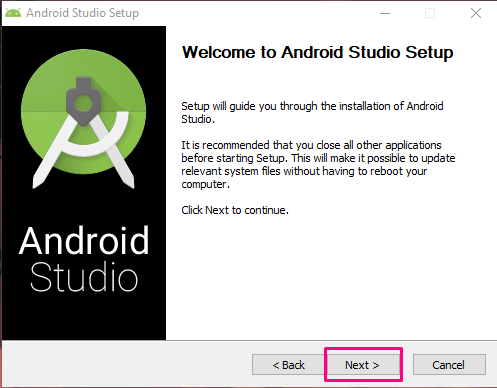
\includegraphics[width=0.48\textwidth]{install_01.png}
		\hfill
		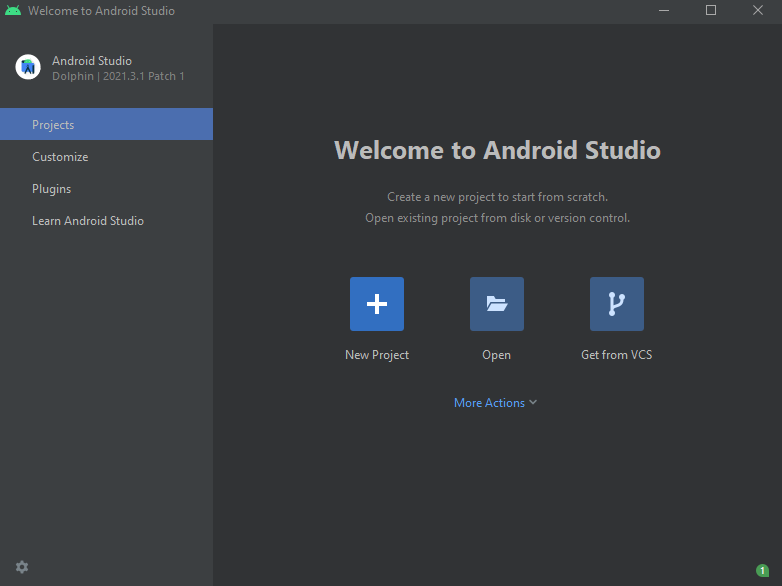
\includegraphics[width=0.48\textwidth]{install_02.png}
		\caption{Instalacija Android Studija - 1. i 2. korak}
		\label{fig:install_01}	
	\end{figure}

	Zatim je potrebno odabrati lokaciju na koju će se instalirati Android studio. Osigurajte da imate dovoljno prostora na lokaciji na koju ga instalirate i ukoliko ste u mogućnosti instalirajte ga na SSD disk. Odabir lokacije prikazan je slikom \ref{fig:install_03}. Što se tiče instalacije samog alata, ona je gotova. Sada je alat potrebno pokrenuti i instalirati dodatne stvari koje su neophodne prilikom razvoja aplikacija. 

	\begin{figure}[!h]
		\centering
		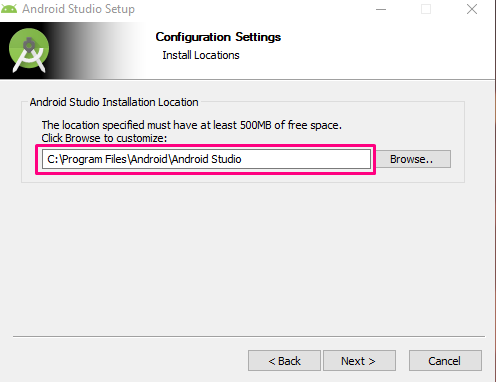
\includegraphics[width=0.5\textwidth]{install_03.png}
			\hfill
		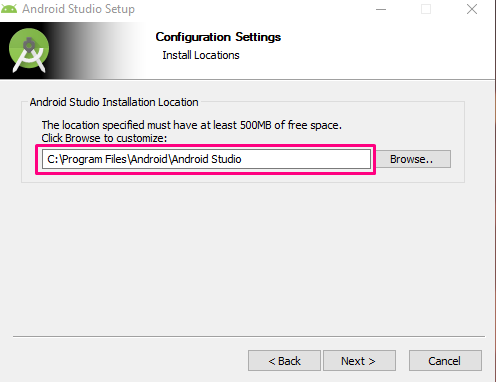
\includegraphics[width=0.48\textwidth]{install_04.png}
		\caption{Instalacija Android Studija - 3. i 4. korak}
		\label{fig:install_03}	
	\end{figure}


	Prilikom pokretanja pojavljuje se čarobnjak koji nudi uvoz postavki iz neke od starijih inačica Android studija. S obzirom da je ovo prvi put kako ga instalirate, ignorirajte ovu opciju. 
	
	\begin{figure}[!h]
		\centering
		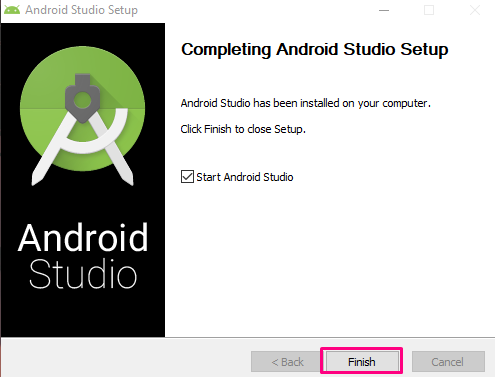
\includegraphics[width=0.3\textwidth]{install_05.png}
		\caption{Instalacija Android Studija - 5. korak}
		\label{fig:install_05}	
	\end{figure}

	S obzirom da postavke nismo uvezli, potrebno je konfigurirati Android studio. Za početak, odaberite želite li slati Googleu anonimnu statistiku o korištenju alata. 	Zatim, odaberite da želite postaviti vlastite postavke, a ne koristiti standardne mogućnosti prilikom instalacije. 	

	\begin{figure}[!h]
		\centering
		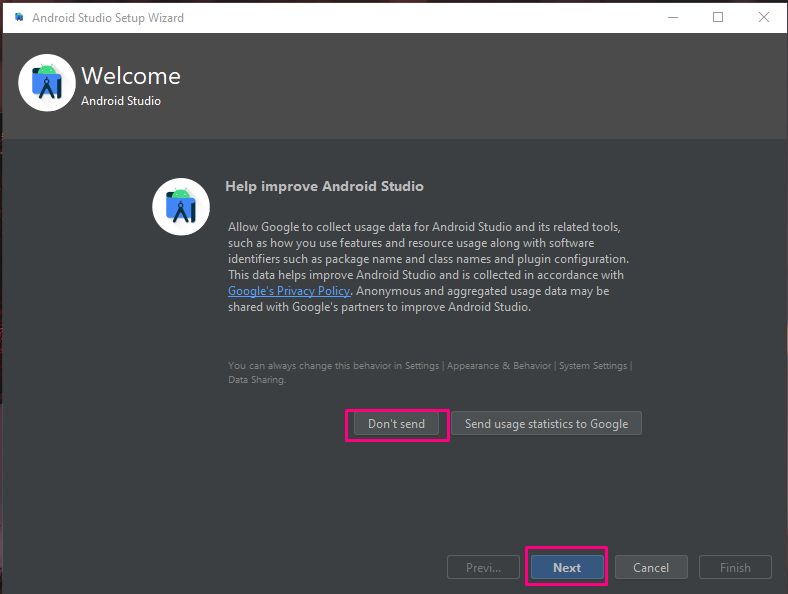
\includegraphics[width=0.48\textwidth]{install_06.png}
		\hfill
		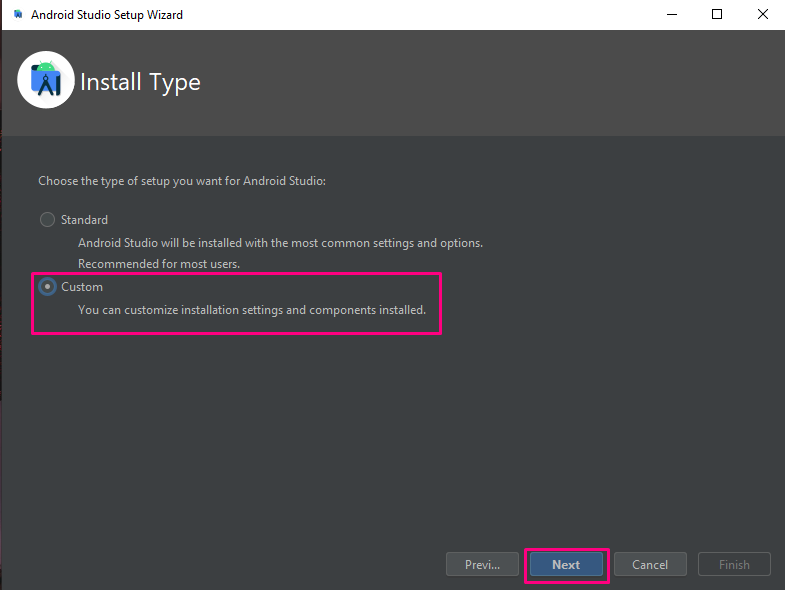
\includegraphics[width=0.48\textwidth]{install_07.png}
		\caption{Instalacija Android Studija - 6. i 7. korak}
		\label{fig:install_06}	
	\end{figure}

	Najprije je potrebno postaviti lokaciju gdje će biti instalirana razvojni paket za programski jezik Javu. Ovo možete ostaviti kako je podrazumijevano, no možete lokaciju i promijeniti, s obzirom da nije nužno da se ona nalazi u instalacijskom direktoriju Android studija, a moguće isti razvojni paket moguće je koristiti i za druge oblike programske podrške. Osim toga, postavlja se tema koja definira izgled razvojnog okruženja. Tamna tema u pravilu je popularnija i ugodnija očima, tako da ju i mi preporučujemo. Ipak, u slučaju da kod pokazujete na projektoru većoj skupini ljudi, svjetla tema se pokazala puno zahvalnijom i praktičnijom radi boljeg kontrasta.
	
	\begin{figure}[!h]
		\centering
		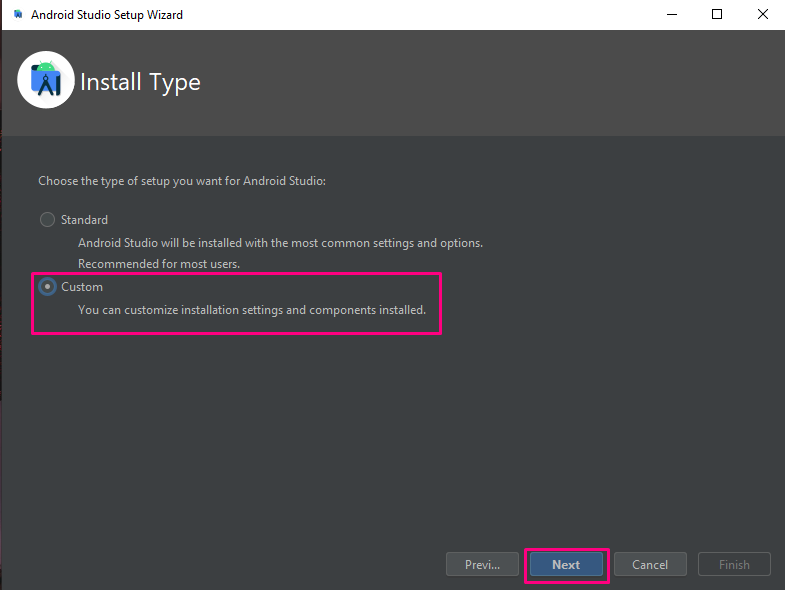
\includegraphics[width=0.48\textwidth]{install_08.png}
		\hfill
		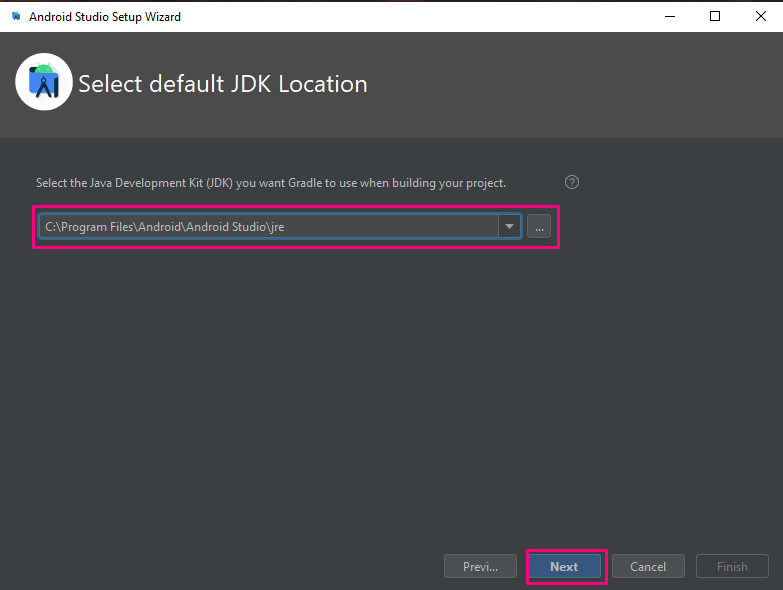
\includegraphics[width=0.48\textwidth]{install_09.png}
		\caption{Instalacija Android Studija - 8. i 9. korak}
		\label{fig:install_08}	
	\end{figure}

	Sljedeće je na redu instalacija Android razvojnog paketa koji sadrži sve klase i alate nužne za nesmetan razvoj aplikacija, Android platforme koju kanite ciljati prilikom razvoja (uobičajeno posljednja koja je dostupna), te Android virtualnog uređaja. Ovo potonje je u stvari emulator, odnosno programsko rješenje koje glumi stvarni uređaj u svakom smislu i trudi se ponašati jednako kako bi se ponašao i stvarni uređaj. Primijetite kako je količina podataka koju je nužno preuzeti doista velika. Opet, nije nužno da se razvojni kit i ostali alati nalaze unutar instalacije Android studija ili da se nalaze u podrazumijevanoj mapi. Slobodno izmijenite lokaciju prilikom instalacije. Na ovom ekranu bit će ponuđene još neke dodatne opcije, primjerice za ubrzavanje emulacije korištenjem odgovarajućih alata namjenjenih procesoru stroja na koji instalirate razvojno okruženje.

	\begin{figure}[!h]
		\centering
		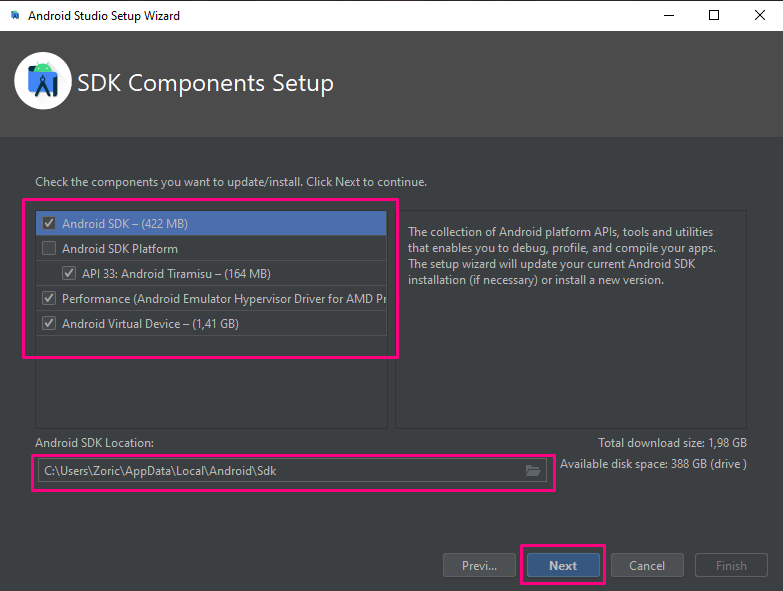
\includegraphics[width=0.48\textwidth]{install_10.png}
		\hfill
		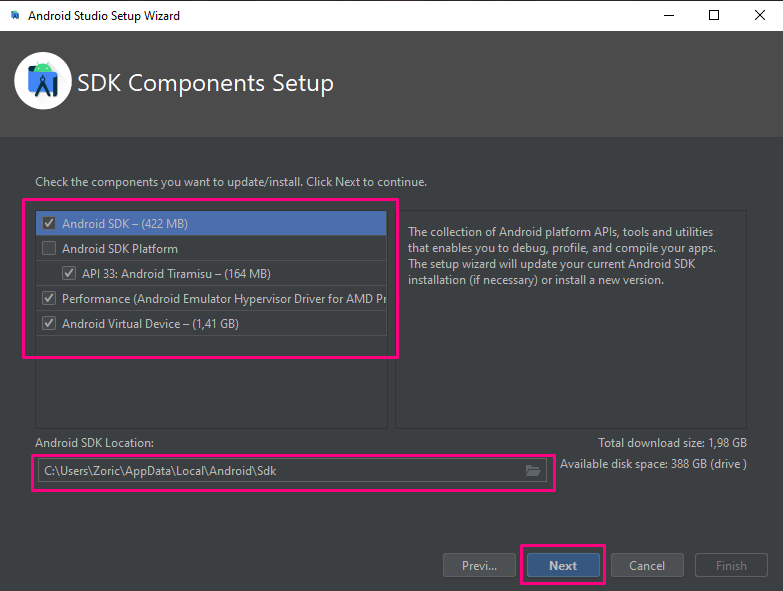
\includegraphics[width=0.48\textwidth]{install_11.png}
		\caption{Instalacija Android Studija - 10. i 11. korak}
		\label{fig:install_10}	
	\end{figure}

	Nakon svega, preostalo je samo provjeriti sve odabrane postavke i potvrditi da prihvaćate uvjete korištenja kako bi se započelo preuzimanje i instalacija svih željenih alata.
		
	\begin{figure}[!h]
		\centering
		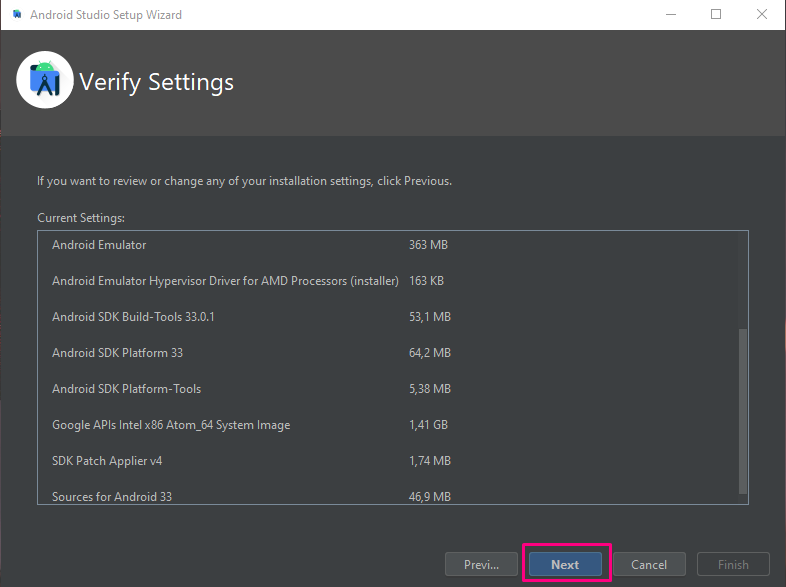
\includegraphics[width=0.48\textwidth]{install_12.png}
		\hfill
		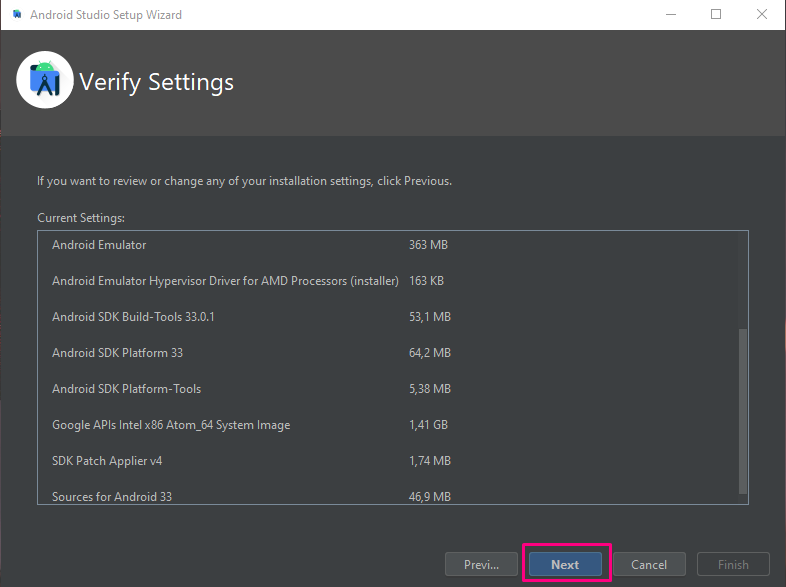
\includegraphics[width=0.48\textwidth]{install_13.png}
		\caption{Instalacija Android Studija - 12. i 13. korak}
		\label{fig:install_12}	
	\end{figure}

	U konačnici, nakon što ste popili kavu (ili 3) dok se sve obavilo, dočekat će vas ekran prikazan slikom \ref{fig:install_14}. Klikom na Finish bit će prikazan početni ekran Android studija na kojem možete kreirati novi projekt ili otvoriti neki od postojećih na kojima ste već ranije radili.
	
	\begin{figure}[!h]
		\centering
		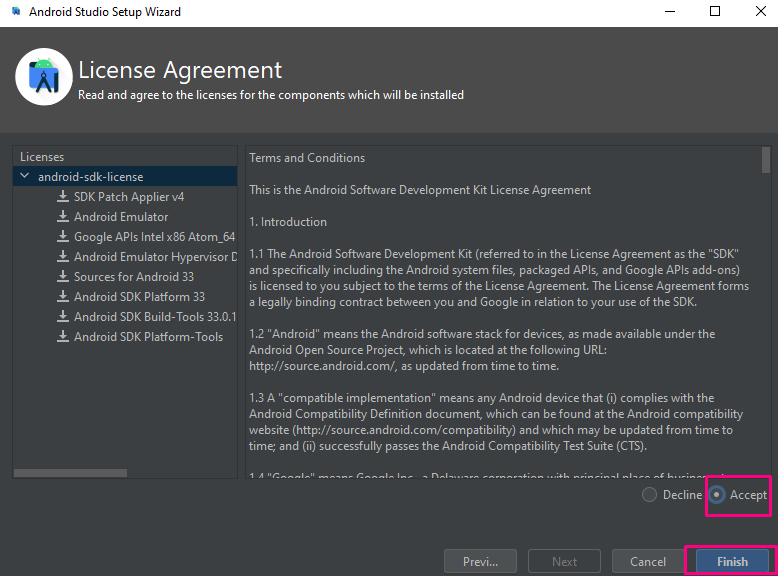
\includegraphics[width=0.48\textwidth]{install_14.png}
		\hfill
		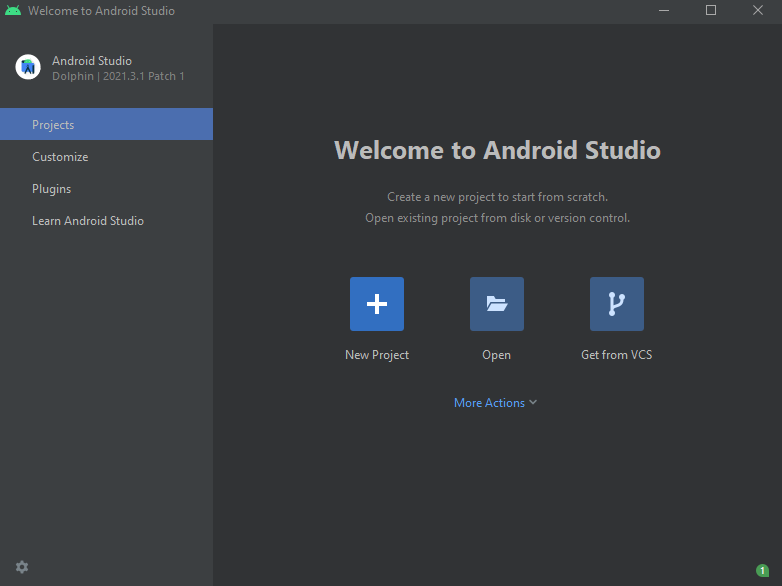
\includegraphics[width=0.48\textwidth]{install_15.png}
		\caption{Instalacija Android Studija - 14. korak}
		\label{fig:install_14}	
	\end{figure}


\section{Kreiranje projekta}

	Kada je razvojno okruženje instalirano, može se pristupiti kreiranju novog projekta. Klikom na gumb \texttt{New Project} kreira se prazan projekt i otvara novi izbornik koji nudi velik broj gotovih predložaka. Svaki od predložaka namijenjen je nekom obliku aplikacije, a vjerojatno ste brojne od njih već vidjeli u aplikacijama koje svakodnevno koristite. Za početak ćemo odabrati platformu za koju želimo raditi aplikaciju iz izbornika. Nude se razne platforme, od telefona do automobila, no mi ćemo odabrati telefone i tablete. Što se tiče predloška, krenut ćemo od najjednostavnije moguće aplikacije s jednim ekranom, a zatim ćemo postupno uvoditi nove ekrane i sadržaj pa stoga odabiremo \texttt{Empty Compose Activity}.
	
	\begin{figure}[!h]
		\centering
		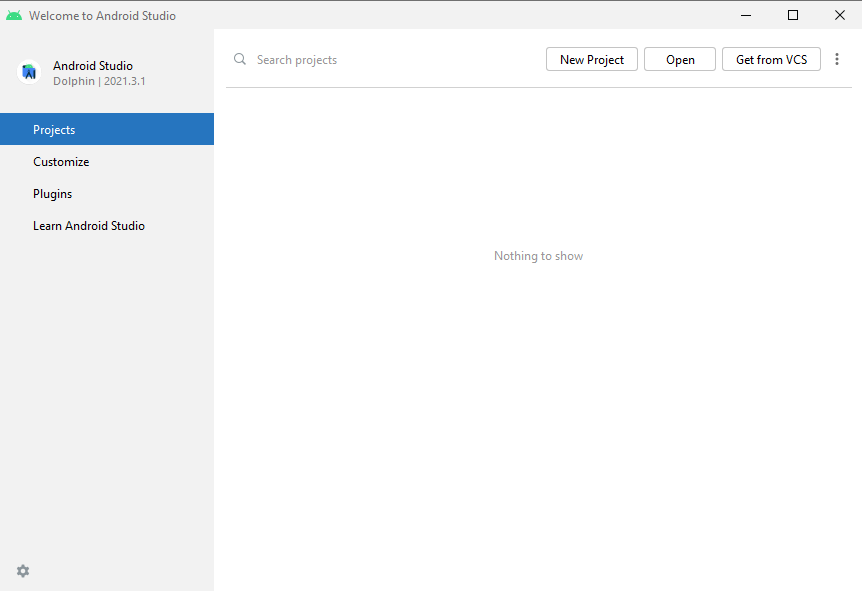
\includegraphics[width=0.48\textwidth]{new_project_01.png}
		\hfill
		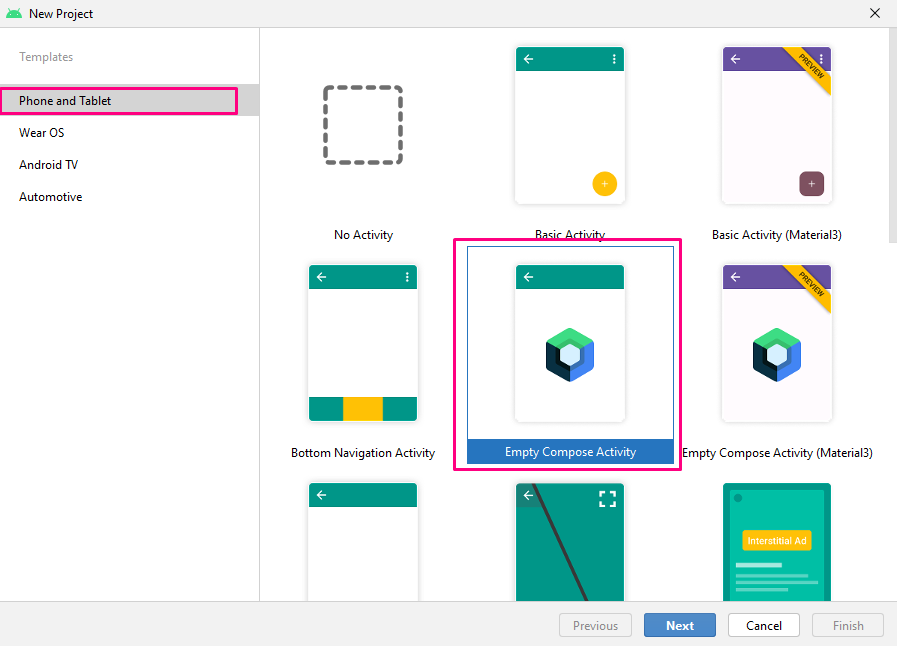
\includegraphics[width=0.48\textwidth]{new_project_02.png}
		\caption{Kreiranje novog projekta - 1. i 2. korak}
		\label{fig:new_project_01}	
	\end{figure}
	
	Kada je odabran željeni predložak, potrebno je unijeti osnovne informacije o aplikaciji. Najprije se unosi ime aplikacije. Riječ je samo o nazivu koji ne mora biti jedinstven, a bilo bi dobro da bude pamtljiv kako bi korisnici Vašu aplikaciju lakše pronašli i dijelili. Zatim se definira ime paketa. Naime, sav kod u programskim jezicima Java i Kotlin koji se mogu rabiti za kreiranje aplikacija za Android platformu razdvaja se po paketima, a potrebno je definirati vršni paket u kojem će biti sav kod. Ovo ime paketa ima još jednu važnu ulogu, ono predstavlja jedinstveni identifikator svake aplikacije u svijetu i mora biti jedinstveno. Preporučuje se stoga uzeti obrnuto ime domene i na kraj dodati ime projekta. Uz to se definira još lokacija gdje će biti pohranjena projkekt na računalu te najstarija inačica Androida na kojoj će biti moguće pokrenuti aplikaciju. Ovisno o najstarijoj inačici koja se odabere, našu aplikaciju moći će skinuti i koristiti više ili manje korisnika, a pružena je korisna poveznica koja u postotcima ukupnih korisnika Androida govori koliko će točno korisnika ona biti dostupna. Novije inačice sustava Android donose nove značajke i poboljšane funkcionalnosti koje ponekad zna biti teško podržati na starijim inačicama. Ovdje svaki programer mora odvagnuti koliko mu je važno dobiti još nekoliko postotaka korisnika u odnosu na cijenu u vremenu i novcu koji za to mora uložiti. Kada je sve spremno, aplikacija se prikazuje u razvojnom okruženju i moguće je započeti s radom.
	
	\begin{figure}[!h]
		\centering
		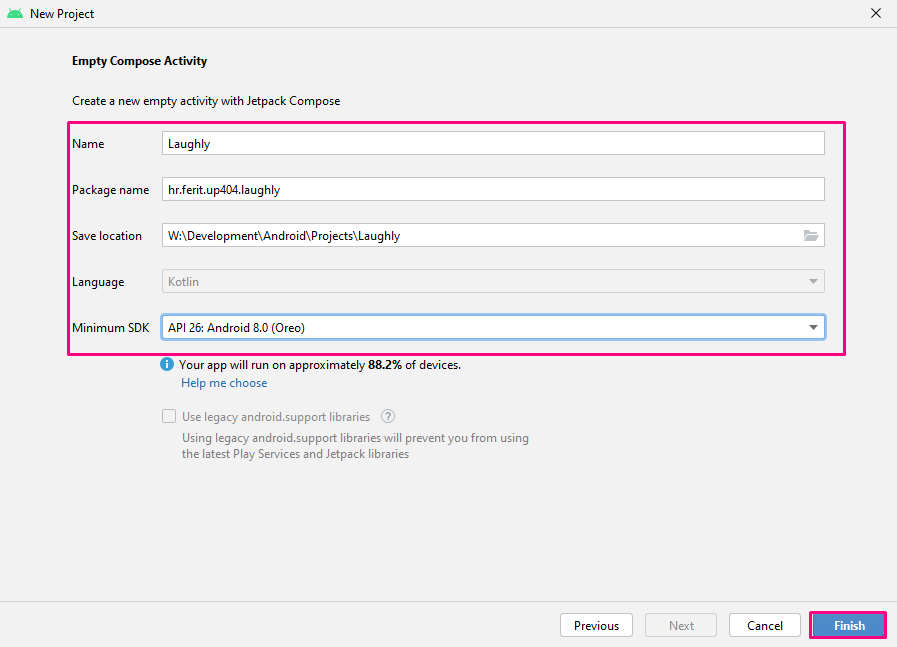
\includegraphics[width=0.48\textwidth]{new_project_03.png}
		\hfill
		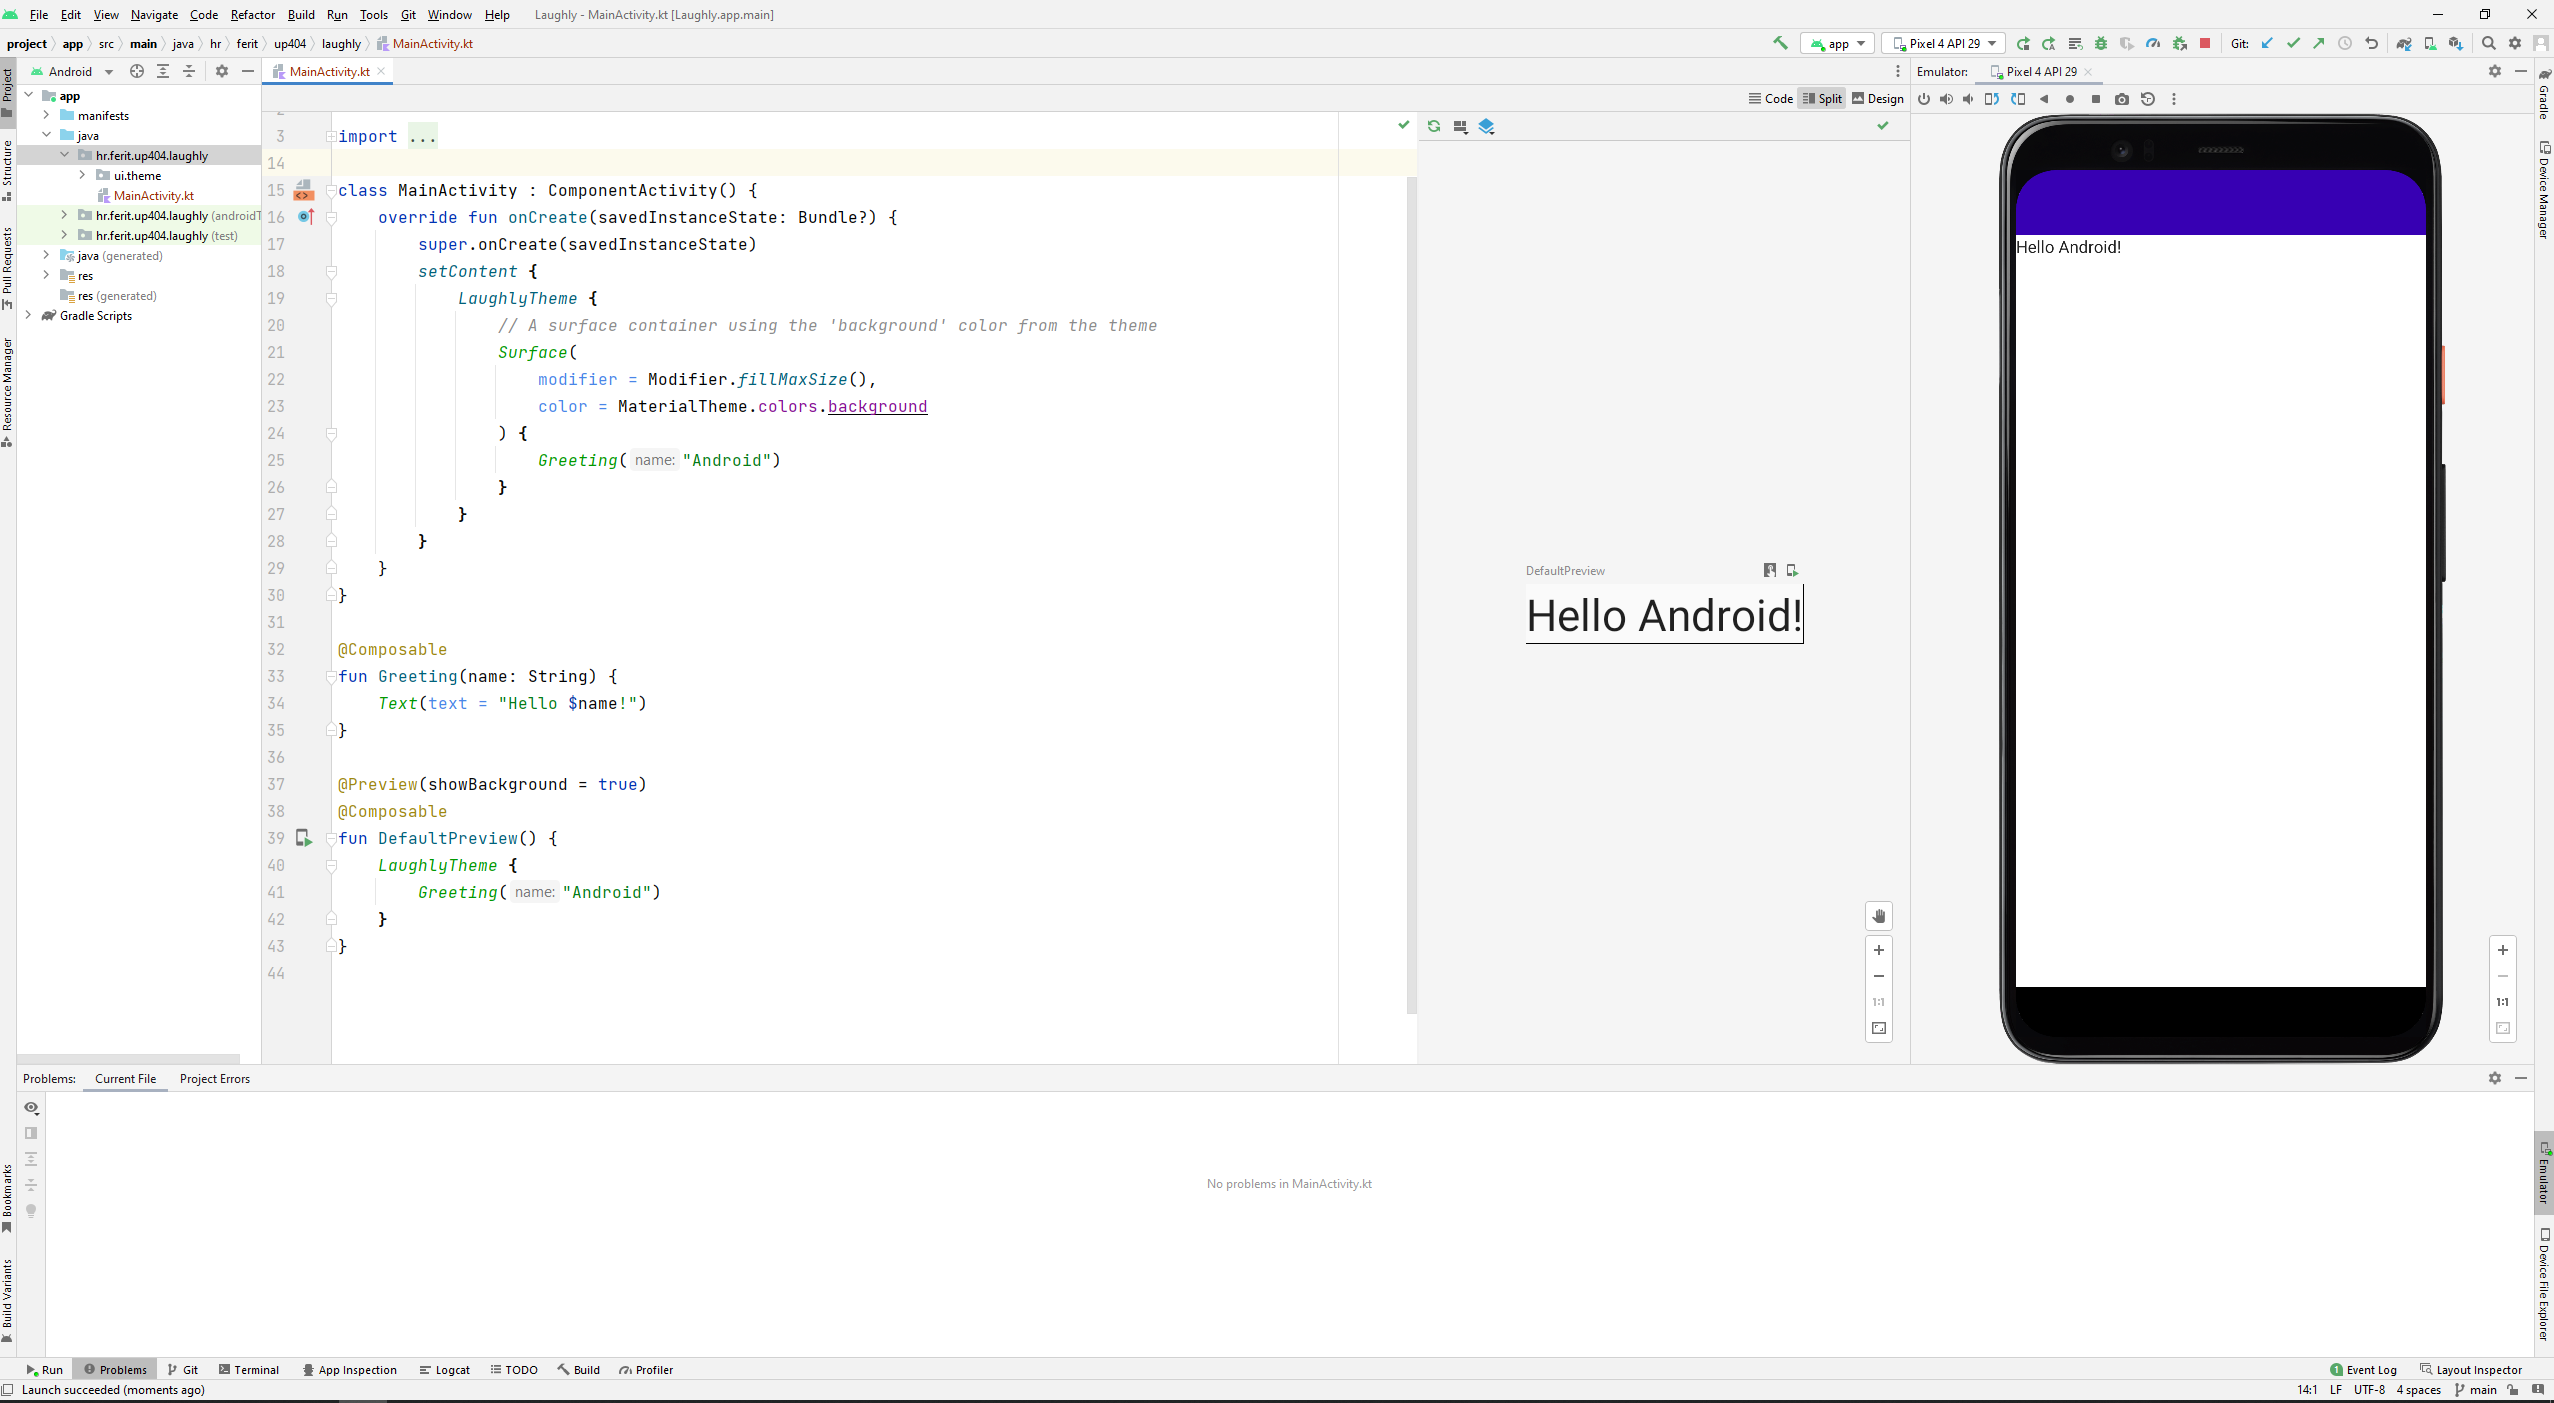
\includegraphics[width=0.48\textwidth]{new_project_04.png}
		\caption{Kreiranje novog projekta - 3. i 4. korak}
		\label{fig:new_project_03}	
	\end{figure}

\section{Uvođenje ekrana i navigacija}

Android aplikacije u pravilu imaju ekrane koji služe za prikaz sadržaja korisniku. Za potrebe prikaza pojedinog ekrana moguće je koristiti rarzličite gotove komponente koje se zovu \texttt{Activity} ili \texttt{Fragment}. Iako je ranije primaran način za oblikovanje i izgradnju korisničkih sučelja bio napisati \texttt{XML} kod koji ih opisuje i koji se vezuje uz pojedini \texttt{Activity} ili \texttt{Fragment}, danas to više nije tako. U novije vrijeme koristi se pristup gdje je svaka komponenta sučelja, uključujući i cijele ekrane, predstavljena funkcijom. Ovo je omogućeno korištenjem biblioteke imena \texttt{Jetpack Compose}, a taj pristup i navedena biblioteka bit će korišteni i u sklopu ove radionice. U ovom slučaju, mora postojati samo jedan \texttt{Activity} koji će služiti kao polazna točka i kontejner za sve ekrane aplikacije. Sama aplikacija imat će pet ekrana. Glavni ekran (\texttt{MainScreen}) sadržavat će komponente za navigaciju i određivati koji je početni ekran aplikacije. Početni ekran (\texttt{HomeScreen}) sadržavat će gumbe za navigaciju prema pojedinim aktivnostima aplikacije. Tri ekrana koja predstavljaju aktivnosti u aplikaciji bit će redom inspirirajući ekran (\texttt{InspireScreen}), zaigrani ekran (\texttt{PlayScreen}) te nasmijani ekran (\texttt{LaughScreen}). 

Prvi korak koji ćemo napraviti je priprema projekta. Prilikom izrade aplikacije za bilo koju platformu programer se oslanja na kod i alate koje su razvili drugi programeri prije njega, a koji dolaze u obliku pripremljenih biblioteka. S obzirom da ih je razvio netko "izvana", često se nazivaju vanjskim ovisnostima (engl. \textit{external dependency}). U suprotnom bi izrada bila osjetno dugotrajnija i zamornija. Kod Android aplikacija, ove se vanjske ovisnosti uključuju u projekt dodavanjem nekoliko linija koda u datoteku \texttt{build.gradle (Module: app)} gdje se opisuje što točno želimo uključiti i koristiti u našem projektu. Sve potrebne vanjske ovisnosti za cjelokupnu radionicu dane su izlistanjem \ref{lst:dependencies}.

\begin{lstlisting}[caption={Ovisnosnosti o vanjskim bibliotekama u datoteci build.gradle (Module:app)}, label={lst:dependencies}, language=Kotlin]
/***********************************************************************/
/*  Specific dependencies for the workshop:*/
/***********************************************************************/
// Navigation with jetpack compose:
def nav_version = "2.5.3"
implementation "androidx.navigation:navigation-compose:$nav_version"

// Ktor for networking:
def ktor_version = '2.2.2'
implementation "io.ktor:ktor-client-core:$ktor_version"
implementation("io.ktor:ktor-client-android:$ktor_version")
implementation "io.ktor:ktor-client-serialization:$ktor_version"
implementation "io.ktor:ktor-serialization-gson:$ktor_version"
implementation("io.ktor:ktor-client-content-negotiation:$ktor_version")
implementation "io.ktor:ktor-client-logging-jvm:$ktor_version"
\end{lstlisting}

Kroz sve ekrane aplikacije koristit ćemo resurse poput boja i dimenzija. Oni se mogu definirati u mapi \texttt{res/values} u odgovarajućim datotekama, a izgled tih datoteka dan je izlistanjem \ref{lst:resources-dimenscolors}.

\begin{lstlisting}[caption={Dimenzije i boje - dimens.xml i colors.xml}, label={lst:resources-dimenscolors}, language=Kotlin]
<!-- dimens.xml -->
<?xml version="1.0" encoding="utf-8"?>
<resources>
	<dimen name="padding_medium">16dp</dimen>
</resources>

<!-- Insert into colors.xml-->
<!-- Custom colors -->
<color name="hotpink">#ef7c8e</color>
<color name="cream">#fae8e0</color>
<color name="spearmint">#b6e2d3</color>
<color name="rosewater">#d8a7b1</color>
\end{lstlisting}

Kako bismo mogli pristupiti organizaciji ekrana naše aplikacije, najprije ćemo definirati sve ekrane i njihove jedinstvene oznake. Ove jedinstvene oznake nazivaju se još i rutama. Ruta predstavlja jedinstvenu oznaku svakog ekrana i omogućuje komponenti za navigaciju da točno zna kamo treba odvesti korisnika. Ove rute definirat ćemo u posebnoj datoteci koju ćemo nazvati \texttt{Navigation.kt}, a koja je prikazana izlistanjem \ref{lst:navigation}.

\begin{lstlisting}[caption={Navigacija - Navigation.kt}, label={lst:navigation}, language=Kotlin]
sealed class Screen(val route: String) {
	object Home : Screen("home")
	object Inspire : Screen("inspire")
	object Laugh : Screen("laugh")
	object Play : Screen("throw")
}
\end{lstlisting}

Svaka funkcija koja predstavlja dio korisničkog sučelja označena je oznakom \texttt{@Composable}. S obzirom da ćemo za početak samo kreirati prazne ekrane za pojedine aktivnosti koje ćemo nadograđivati i popunjavati sadržajem kako radionica bude odmicala, kreirajmo redom sva tri ekrana za aktivnosti, prema izlistanjima \ref{lst:screen-inspire}, \ref{lst:screen-play}, \ref{lst:screen-laugh}. Svaki od ovih ekrana kreira se u zasebnoj datoteci čije ime odgovara imenu ekrana, dakle \texttt{InspireScreen, PlayScreen, LaughScreen}.

\begin{lstlisting}[caption={Inspirirajući ekran - InspireScreen.kt}, label={lst:screen-inspire}, language=Kotlin]
@Composable
fun InspireScreen() {
	 Text(text = "Inspire screen")
}
\end{lstlisting}
\begin{lstlisting}[caption={Zaigrani ekran - PlayScreen.kt}, label={lst:screen-play}, language=Kotlin]
	@Composable
	fun PlayScreen() {
		Text(text = "Play screen")
	}
\end{lstlisting}
\begin{lstlisting}[caption={Nasmijani ekran - LaughScreen.kt}, label={lst:screen-laugh}, language=Kotlin]
	@Composable
	fun LaughScreen() {
		Text(text = "Laugh screen")
	}
\end{lstlisting}

Idući korak je kreiranje početnog ekrana. Riječ je o ekranu koji će sadržavati gumbe koji će korisniku omogućiti odlazak na neki od ranije pripremljenih ekrana u aplikaciji. Izgled početnog ekrana dan je izlistanjem \ref{lst:home-screen}. Ovaj je ekran nešto kompleksniji od dosadašnjih. Vidimo da, kako bi taj ekran radio, traži od nas da mu damo \texttt{NavController}. Riječ je o komponenti za navigaciju koju ćemo pripremiti kasnije i predati ju početnom ekranu svaki put kada ga zatrebamo. Osim toga, sučelje ovog ekrana sadrži više sadržaja no prethodni ekrani. Za kreiranje sučelja koriste se druge \texttt{Composable} funkcije koje pozivamo unutar naše funkcije \texttt{HomeScreen()}. Najprije, želimo kreirati kontejner za sav sadržaj i postaviti mu pozadinsku sliku. Ovo postižemo funkcijom \texttt{Box()} i postavljanjem slike kao prvog elementa u nju (poziv funkciji \texttt{Image()}). Uz sliku, funkcija \texttt{Box()} sadržavat će i stupac s gumbima, za što se koristi funkcija \texttt{Column()}. Unutar potonje iskoristit će se tri poziva funkciji \texttt{NavigateButton()} koju smo sami definirali u datoteci \texttt{NavigateButton.kt}. Naime, čest je slučaj da se pojedine komponente koriste na više mjesta. Kako bi se izbjeglo ponavljanje koda na svim tim mjestima (npr. postavljanje boje, veličine teksta i slično), moguće je definirati komponentu zasebno u obliku funkcije sa željenim vrijednostima ovih postavku i onda ju pozvati gdje god je ona potrebna. Navigacijski gumb definiran je u datoteci \texttt{NavigateButton.kt}, a izgled je dan izlistanjem koda \ref{lst:navigate-button}.

\begin{lstlisting}[caption={Početni ekran - HomeScreen.kt}, label={lst:screen-home}, language=Kotlin]
@Composable
fun HomeScreen(navController: NavController) {
	Box(modifier = Modifier.fillMaxSize()) {
		Image(
		painter = painterResource(id = R.drawable.background),
		contentDescription = "Background gradient image",
		modifier = Modifier.matchParentSize(),
		contentScale = ContentScale.Crop
		)
		Column(
		modifier = Modifier.fillMaxSize(),
		verticalArrangement = Arrangement.Center,
		horizontalAlignment = Alignment.CenterHorizontally		
		) {
			NavigateButton(
			text = stringResource(id = R.string.label_inspire),
			onClick = { navController.navigate(Screen.Inspire.route) }
			)
			NavigateButton(
			text = stringResource(id = R.string.label_laugh),
			onClick = { navController.navigate(Screen.Laugh.route) }
			)
			NavigateButton(
			text = stringResource(id = R.string.label_play),
			onClick = { navController.navigate(Screen.Play.route) }
			)
		}
	}
}
\end{lstlisting}

\begin{lstlisting}[caption={Gumb za navigaciju - NavigateButton.kt}, label={lst:navigate-button}, language=Kotlin]
@Composable
fun NavigateButton(text: String, onClick: () -> Unit) {
	Button(
	onClick = onClick,
	Modifier.padding(dimensionResource(id = R.dimen.padding_medium)),
	colors = ButtonDefaults.buttonColors(
	backgroundColor = colorResource(id = R.color.rosewater),
	contentColor = colorResource(id = R.color.cream)
	)
	) {
		Text(text = text, fontSize = 20.sp)
	}
}
\end{lstlisting}

Kada je sve ostalo pripremljeno, potrebno je sve i povezati u cjelinu i to kreiranjem glavnog ekrana. Za kreiranje glavnog ekrana rabi se stoga funkcija dana izlistanjem \ref{lst:screen-main}. U toj funkciji kreirana je komponenta za navigaciju kroz aplikaciju te je navedeno koji ekran je početni, a koji su ekrani na koje je moguće navigirati. Možete primijetiti da se ovdje kreira i postavlja navigacijska komponenta koja je potrebna početnom ekranu aplikacije.

\begin{lstlisting}[caption={Glavni ekran - MainScreen.kt}, label={lst:screen-main}, language=Kotlin]
@Composable
fun MainScreen() {
	val navController = rememberNavController()
	NavHost(navController = navController, startDestination = Screen.Home.route) {
		composable(Screen.Home.route) { HomeScreen(navController) }
		composable(Screen.Laugh.route) { LaughScreen() }
		composable(Screen.Inspire.route) { InspireScreen() }
		composable(Screen.Play.route) { PlayScreen() }
	}
}
\end{lstlisting}

Preostalo je još samo reći Android sustavu da, kada se pokrene aplikacija, prikaže najprije glavni ekran (ovaj nema sadržaja) koji će onda odmah navigirati ka početnom ekranu. Ovo se postiže izmjenom linije koda u datoteci \texttt{MainActivity.kt} prema izlistanju \ref{lst:main-activity} tako da se poziva ranije definirana funkcija \texttt{MainScreen()}.

\begin{lstlisting}[caption={Glavna aktivnost - MainActivity.kt}, label={lst:activity-main}, language=Kotlin]
class MainActivity : ComponentActivity() {
	override fun onCreate(savedInstanceState: Bundle?) {
		super.onCreate(savedInstanceState)
		
		setContent {
			LaughlyTheme {
				// A surface container using the 'background' color from the theme
				Surface(
				modifier = Modifier.fillMaxSize(),
				color = MaterialTheme.colors.background
				) {
					MainScreen()
				}
			}
		}
	}
}
\end{lstlisting}

% TODO: Dodati link na jetpack compose.

\section{Značajka - inspiracija}

Kao prvu aktivnost koju nudimo unutar naše aplikacije, omogućit ćemo korisnicima da se inspiriraju poznatom osobom koja je za nas inspirativna. Na radionici možete samostalno odabrati osobu koju želite, prikupiti potrebne materijale i zatim iskoristiti upute i kod dan na ovim stranicama kako biste aplikaciju učinili osobnijom. 

Krenut ćemo s informacijom da je fiksni sadržaj u Android aplikacijama izdvojen u datoteke za specifične oblike sadržaja. Primjerice, tekst koji prikazujete na gumbima, dimenzije margina ili slike koje predstavljaju fiksne grafičke elemente u aplikacijama izdvajaju se izvan koda aplikacije. Razlog je taj što iz brojnih razloga u nekim situacijama trebate drugačiji izgled ili prikaz. Primjerice, korisnici u Njemačkoj očekuju sadržaj na njemačkom jeziku, dok bi stanovnicima Hrvatske to predstavljalo problem i oni očekuju hrvatski jezik. Svaka vrijednost koju kanite rabiti predstavljena je resursom koji ima jedinstveni identifikator. Ovo omogućuje programeru da koristi resurs preko identifikatora, a prepusti sustavu da, ovisno o postavkama sustava, brine o tome koji će se konkretan resurs učitati. Tekst se tako izdvaja u datoteku \texttt{strings.xml} koja je smještena u direktorij \texttt{res/values}. Cjelokupni izgled ove datoteke dan je izlistanjem \ref{lst:strings} i uključuje tekst za cijelu aplikaciju.

\begin{lstlisting}[caption={Resursi - values/strings.xml}, label={lst:resources-strings}, language=Kotlin]
<resources>
<string name="app_name">Laughly</string>
<!-- Custom strings: -->
<string name="label_inspire">Get inspired!</string>
<string name="label_laugh">Laugh!</string>
<string name="label_play">Play!</string>
<string name="label_quote">Quote</string>
<string name="name_turing">Alan Turing</string>
<string name="info_turing">"He was the most important mathematician of the second world war. He helped to break the German's Enigma code at Blatchley Park, by designing a computer to decipher the German messages called the Bombe. The most important effects of this revolutionary invention were:\n - Shortening the length of the war: by decoding the German's messages Blatchley Park's team was able to identify the position of all Nazi's boats so the Royal Navy was able to protect English naval fleet from u-boats's attacks.\n - Saving millions lives: the avoided attacks permit a lot of people to stay in life. Turing's team, on the other hand, had to avoid that German discover that  Enigma had been decrypted. An electromechanical device that helped the code-breakers to calculate the key of the day the German were using on their Enigma machine.Using a menu provided by the codebreaking team from a crib (plaintext that corresponded to ciphertext), the Bombe operators could quickly set up the machine and let it calculate possible Enigma settings.\n  After the war Alan Turing came up with Turing Test, a method to test artificial intelligence.Persecuted for homosexual acts, he committed suicide in 1954.\n"</string>
<string name="quote_turing_1">Sometimes it is the people no one imagines anything of who do the things that no one can imagine.</string>
<string name="quote_turing_2">A computer would deserve to be called intelligent if it could deceive a human into believing that it was human.</string>
<string name="quote_turing_3">Unless in communicating with it one says exactly what one means, trouble is bound to result.</string>
<string name="label_reroll">Re-roll</string>
<string name="description_joke_icon">New joke icon</string>
<string name="label_refresh_joke">Get new joke!</string>
</resources>
\end{lstlisting}

Sadržaj koji će biti prikazan u Android aplikacijama uobičajeno se ne definira unutar ekrana koji definira kako će sadržaj izgledati (razdvajanje prezentacije od implementacije). Za potrebe razdvajanja ovog sadržaja, ali i ostvarivanje brojnih drugih prednosti, koriste se komponente koje se nazivaju \texttt{ViewModel}. Tijekom radionice kreirat ćemo odgovarajuće \texttt{ViewModel} komponente za svaki ekran aplikacije. Za \texttt{InspireScreen} taj je \texttt{ViewModel} dan izlistanjem \ref{lst:vm-inspire}. Može se uočiti kako taj \texttt{ViewModel} referencira resurse koje ćemo unutar ekrana iskoristiti za prikaz sadržaja te omogućuje da se dohvati resurs nasumičnog citata u bilo kojem trenutku kroz funkciju \texttt{getQuote()}.

\begin{lstlisting}[caption={Inspirirajući \texttt{view model}- InspireViewModel.kt}, label={lst:viewmodel-inspire}, language=Kotlin]
class InspireViewModel : ViewModel() {
	
	val name = R.string.name_turing
	val info = R.string.info_turing
	val image = R.drawable.turing
	private val quotes = listOf<Int>(
		R.string.quote_turing_1,
		R.string.quote_turing_2,
		R.string.quote_turing_3
	)
	
	fun getQuote() = quotes.random()
}
\end{lstlisting}

Jednom kada je \texttt{ViewModel} definiran, pristupamo definiranju ekrana koji ga rabi. U ovom slučaju je riječ o inspirirajućem ekranu \texttt{InspireScreen}. Inspire screen sastoji se od nekolicine komponenti koje omogućuju prikaz svog sadržaja smještenog unutar ranije danog \texttt{ViewModel}-a. Sam \texttt{ViewModel} ubacuje se u ekran svaki put kada ga je potrebno prikazati, a za te potrebe rabi se funkcija \texttt{viewModel()}. 

\begin{lstlisting}[caption={Inspirirajući ekran - InspireScreen.kt}, label={lst:screen-inspire-final}, language=Kotlin]
@Composable
fun InspireScreen(viewModel: InspireViewModel = viewModel()) {
	Column(
		modifier = Modifier.fillMaxSize()
		.background(colorResource(id = R.color.cream))
		.padding(dimensionResource(id = R.dimen.padding_medium))
	) {
		Row(
			verticalAlignment = Alignment.CenterVertically,
			horizontalArrangement = Arrangement.Center,
			modifier = Modifier.weight(1f)
		) {
			Image(
				painter = painterResource(id = viewModel.image),
				contentDescription = stringResource(id = viewModel.name),
				contentScale = ContentScale.Crop,
				modifier = Modifier.size(100.dp, 100.dp).clip(CircleShape)
			)
			Text(
				text = stringResource(viewModel.name),
				fontSize = 48.sp,
				textAlign = TextAlign.Center,
				color = colorResource(id = R.color.rosewater),
				modifier = Modifier.fillMaxWidth()
			)
		}
		Text(
			text = stringResource(id = viewModel.info),
			fontSize = 14.sp,
			modifier = Modifier
			.weight(3f)
			.fillMaxWidth()
			.padding(dimensionResource(id = R.dimen.padding_medium))
		)
		Column(
			horizontalAlignment = Alignment.CenterHorizontally,
			verticalArrangement = Arrangement.SpaceEvenly,
			modifier = Modifier.weight(1f)
		) {
			var quoteResourceId by remember { mutableStateOf(viewModel.getQuote()) }
			Text(
				text = stringResource(id = quoteResourceId),
				fontSize = 16.sp,
				textAlign = TextAlign.Center,
				color = colorResource(id = R.color.hotpink),
				modifier = Modifier.fillMaxWidth()
			)
			Button(onClick = { quoteResourceId = viewModel.getQuote() }) {
				Text(text = stringResource(R.string.label_quote))
			}
		}
	}
}
\end{lstlisting}

\section{Značajka - igra}

Kao drugu aktivnost koju nudimo unutar aplikacije, omogućit ćemo korisnicima da bacaju kockice za Jamb. Kako bismo ostvarili ovu funkcionalnost, dizajnirat ćemo jedan ekran aplikacije tako da prikazuje šest kockica za Jamb te mu dodati gumb ispod kockica klikom na koji će se izgenerirati slučajni brojevi koji će biti prikazani u obliku sličica kockica. Kasnije ćemo dodati funkcionalnost da se promjenom vrijednosti na senzoru akceleracije, primjerice trešnjom uređaja, okine bacanje kockica. Kao prvi korak, preuzet ćemo sličice kockica s Interneta i postaviti ih u mapu \texttt{res/drawable} i to tako da ime svake kockice bude slovo \texttt{d} popraćeno brojem koji kockica prikazuje. Kao idući korak, kreirat ćemo jednu komponentu sučelja koja će prikazivati šest kockica, prema izlistanju \ref{lst:component-dice}. Ovu komponentu smjestit ćemo u paket \texttt{ui/components} gdje držimo sve zasebne komponente koje smo samostalno kreirali. Uočite u izlistanju koda da smo definirali posebnu funkciju koja zna prevesti iz broja koji se treba prikazati na kockici u identifikator sličice koja predstavlja taj broj. Ovo smo napravili kako tu logiku ne bismo morali ponavljati svuda gdje se koristi kockica.

\begin{lstlisting}[caption={Komponenta kockice - Dice.kt}, label={lst:component-dice}, language=Kotlin]
@Composable
fun Dice(values: List<Int>) {
	Column {
		Row(
		horizontalArrangement = Arrangement.SpaceEvenly,
		verticalAlignment = Alignment.CenterVertically,
		modifier = Modifier.fillMaxWidth()
		) {
			Image(
			painter = painterResource(id = GetDiceDrawableId(values[0])),
			contentDescription = "Icon 1"
			)
			Image(
			painter = painterResource(id = GetDiceDrawableId(values[1])),
			contentDescription = "Icon 1"
			)
			Image(
			painter = painterResource(id = GetDiceDrawableId(values[2])),
			contentDescription = "Icon 1"
			)
		}
		Spacer(modifier = Modifier.size(16.dp))
		Row(
		horizontalArrangement = Arrangement.SpaceEvenly,
		verticalAlignment = Alignment.CenterVertically,
		modifier = Modifier.fillMaxWidth()
		) {
			Image(
			painter = painterResource(id = GetDiceDrawableId(values[3])),
			contentDescription = "Icon 1"
			)
			Image(
			painter = painterResource(id = GetDiceDrawableId(values[4])),
			contentDescription = "Icon 1"
			)
			Image(
			painter = painterResource(id = GetDiceDrawableId(values[5])),
			contentDescription = "Icon 1"
			)
		}
	}
}
fun GetDiceDrawableId(value: Int): Int {
	return when (value) {
		1 -> R.drawable.d1
		2 -> R.drawable.d2
		3 -> R.drawable.d3
		4 -> R.drawable.d4
		5 -> R.drawable.d5
		6 -> R.drawable.d6
		else -> R.drawable.d1
	}
}
\end{lstlisting}

Kada smo pripremili prikaz za kockice, dodat ćemo tu komponentu na ekran, a dodat ćemo i ranije spomenuti gumb. 

\begin{lstlisting}[caption={Ekran za igru - PlayScreen.kt}, label={lst:screen-play}, language=Kotlin]
@Composable
fun PlayScreen(viewModel: PlayViewModel = viewModel()) {
	val values by viewModel.numbers.collectAsState()
	
	Column(
	verticalArrangement = Arrangement.SpaceEvenly,
	horizontalAlignment = Alignment.CenterHorizontally,
	modifier = Modifier
	.fillMaxSize()
	.background(colorResource(id = R.color.cream))
	.padding(dimensionResource(id = R.dimen.padding_medium))
	) {
		Dice(values)
		Button(onClick = { viewModel.randomize() }) {
			Icon(
			imageVector = Icons.Default.Refresh,
			contentDescription = stringResource(R.string.label_reroll)
			)
			Text(text = stringResource(id = R.string.label_reroll))
		}
	}
}
\end{lstlisting}

Kao i u ranijem slučaju ekrana za inspiraciju, definirat ćemo posebnu klasu koja će služiti za pohranu podataka i pisanje logike iza prikaza, a koja se naziva modelom pogleda (engl. \textit{view model}). Već je sada uočljivo kako imamo listu brojeva koju prikazujemo, kao i da postoji funkcionalnost za ponovno bacanje kockica, odnosno generiranje nasumičnih vrijednosti. Ova funkcionalnost vezana je uz klik gumba. Dodatna funkcionalnost vezana uz senzore na Android platformi ostvaruje se tako da se koristi upravitelj senzorima i preko njega dođe do željenog objekta klase \texttt{Sensor}. Jednom kada je senzor dohvaćen (ako postoji). moguće je prijaviti alat za osluškivanje promjena vrijednosti koje taj senzor mjeri.

\begin{lstlisting}[caption={Model pogleda za igru - PlayViewModel.kt}, label={lst:viewmodel-play}, language=Kotlin]
class PlayViewModel : ViewModel() {
	val numbers = MutableStateFlow(listOf(1, 1, 1, 1, 1, 1))
	private val context = Laughly.application
	private val sensorManager = context.getSystemService(Context.SENSOR_SERVICE) as SensorManager
	private val accelerationSensor = sensorManager.getDefaultSensor(Sensor.TYPE_ACCELEROMETER)
	private val accelerationThreshold = 12
	private val sensorEventListener = object : SensorEventListener {
		override fun onSensorChanged(event: SensorEvent?) {
			event?.let {
				val total = event.values.map { it * it }.sum()
				if (sqrt(total) > accelerationThreshold) {
					randomize()
				}
			}
		}
		override fun onAccuracyChanged(p0: Sensor?, p1: Int) {}
	}
	init {
		if (context.packageManager.hasSystemFeature(PackageManager.FEATURE_SENSOR_ACCELEROMETER)) {
			accelerationSensor?.let {
				sensorManager.registerListener(
				sensorEventListener,
				accelerationSensor,
				SensorManager.SENSOR_DELAY_UI
				)
			}
		}
	}
	fun randomize() {
		val rolled = mutableListOf<Int>()
		repeat(6) {
			rolled.add(Random.nextInt(1, 7))
		}
		numbers.value = rolled
	}
}
\end{lstlisting}

Još je jedan detalj preostao kako bi omogućili rad sa senzorima, a to je definirati klasu koja predstavlja aplikaciju. Ovu klasu nazvat ćemo \texttt{Laughly} i u nju smjestiti kod prikazan izlistanjem \ref{lst:app-laughly}. Ovo je važno jer kad god se pristupa sustavskim uslugama na Android platforme, to se ostvaruje preko nečeg što se naziva kontekts. Riječ je o objektu koji zna sve o trenutnoj okolini aplikacije koja se izvodi i pruža pristupne točke prema sustavskim uslugama. Osim kreiranja klase \texttt{Laughly}, u datoteku \texttt{AndroidManifest.xml} potrebno je dodati liniju koda kako bismo tu novu klasu uistinu registrirali kao aplikacijsku klasu. To se postiže dodavanjem atributa \texttt{name} unutar oznake \texttt{application} u manifest datoteci.

\begin{lstlisting}[caption={Aplikacijska klasa - Laughly.kt}, label={lst:app-laughly}, language=Kotlin]
class Laughly : Application() {
	companion object {
		lateinit var application: Application
	}
	override fun onCreate() {
		super.onCreate()
		application = this
	}
}	
\end{lstlisting}

\begin{lstlisting}[caption={Manifest datoteka - AndroidManifest.xml}, label={lst:manifest}, language=Kotlin]
<?xml version="1.0" encoding="utf-8"?>
<manifest xmlns:android="http://schemas.android.com/apk/res/android"
	xmlns:tools="http://schemas.android.com/tools">
	<uses-permission android:name="android.permission.INTERNET"/>
	<application
		android:name=".Laughly"
		<!-- ... -->
\end{lstlisting}

\section{Značajka - šala}

Konačna funkcionalnost aplikacije bit će nasmijavanje korisnika. Ovo ćemo postići tako da korisnik ode na ekran za smijanje, klikne gumb i time dobije prikaz nasumične šale. Bit će riječ o jednostavnim šalama, na engleskom jeziku, koje se sastoje od dva dijela - postavke (engl. \textit{setup}) i vica (engl. \textit{punchline}). Kako ne bismo sami sastavljali brojne viceve, poslužit ćemo se servisom koji je dostupan na Internetu i od kojeg ćemo zatražiti da nam da novi vic, svaki put kada mi pošaljemo upit prema njemu. Upit ćemo izvesti putem protokola HTTP, a odgovor ćemo dobiti zapakiran u oblik JSON. Ove Vas kratice ne trebaju pretjerano brinuti, riječ je o standardiziranim načinma i formatima komunikacije između aplikacija. Sam servis smješten je na adresi \url{https://official-joke-api.appspot.com/random_joke}. Možete pokušati na navedenu adresu otići uporabom internetskog preglednika i primijetit ćete da svaki put kada osvježite stranicu, dobijete novu šalu. S obzirom da uvodimo pojmove poput šale i servisa za šale, krenut ćemo implementirati s te strane. Naučit ćemo naš programski jezik te pojmove tako što ćemo mu ih opisati korištenjem klasa. U paket \texttt{laughing} dodat ćemo dvije nove Kotlin klase, \texttt{Joke} i \texttt{JokeApiService}.

\begin{lstlisting}[caption={Klasa Joke - Joke.kt}, label={lst:Joke}, language=Kotlin]
data class Joke(
	val setup: String,
	val punchline: String
)
\end{lstlisting}

\begin{lstlisting}[caption={Klasa JokeApiService - JokeApiService.kt}, label={lst:JokeApiService}, language=Kotlin]
class JokesApiService {
	private val client = HttpClient(Android) {
		install(DefaultRequest) {
			headers.append("Content-Type", "application/json")
		}
		install(ContentNegotiation) {
			gson {
				setPrettyPrinting()
			}
		}
		engine {
			connectTimeout = 60_000
			socketTimeout = 60_000
		}
	}
	suspend fun getJoke(): Joke {
		return client.get("https://official-joke-api.appspot.com/random_joke").body()
	}
}	
\end{lstlisting}

Prikaz šale na ekranu nije kompliciran, zapravo se sastoji od dva tekstualna elementa i jednog gumba koji osvježava prikaz postavke i vica.

\begin{lstlisting}[caption={Ekran šale - LaughScreen.kt}, label={lst:screen-laugh}, language=Kotlin]
@Composable
fun LaughScreen(viewModel: LaughViewModel = viewModel()) {
	Column(
	verticalArrangement = Arrangement.SpaceEvenly,
	horizontalAlignment = Alignment.CenterHorizontally,
	modifier = Modifier
	.fillMaxSize()
	.background(colorResource(id = R.color.cream))
	.padding(dimensionResource(id = R.dimen.padding_medium))
	) {
		val joke by viewModel.joke.collectAsState()
		Text(
		text = joke.setup,
		fontSize = 32.sp,
		textAlign = TextAlign.Center
		)
		Text(
		text = joke.punchline,
		fontSize = 32.sp,
		textAlign = TextAlign.Center
		)
		Button(onClick = { viewModel.updateJoke() }) {
			Image(
			painterResource(id = android.R.drawable.ic_menu_more),
			contentDescription = stringResource(R.string.description_joke_icon),
			modifier = Modifier.size(20.dp)
			)
			Text(
			text = stringResource(R.string.label_refresh_joke),
			Modifier.padding(start = 10.dp)
			)
		}
	}
}
\end{lstlisting}

Preostalo je još samo definirati model prikaza za dani ekran unutar kojeg će biti sačuvana trenutna šala i omogućeno dohvaćanje nove šale.

\begin{lstlisting}[caption={Model prikaza šale - LaughViewModel.kt}, label={lst:viewmodel-laugh}, language=Kotlin]
class LaughViewModel : ViewModel() {
	private val apiService = JokesApiService()
	val joke = MutableStateFlow(Joke("", ""))
	init {
		updateJoke()
	}
	fun updateJoke() {
		viewModelScope.launch {
			joke.value = apiService.getJoke()
		}
	}
}
\end{lstlisting}

\section{Što dalje?}

	\begin{itemize}
		\item Android app fundamentals: \url{https://developer.android.com/courses/fundamentals-training/toc-v2}
		\item Android kolegij \url{https://www.udacity.com/course/android-kotlin-developer-nanodegree--nd940youtube }
		\item Besplatan kolegij \url{https://www.youtube.com/watch?v=fis26HvvDII}
	\end{itemize}


	

\end{document}

